\chapter{Implementation, Results and Discussion}\label{ch:results}
This chapter describes the implementation, then reports results for each layer: the corpus, the historical analysis,
the topic classifier, paper generation, the assistant and the deployed application.

\section{Implementation and Requirements}
PaperMind is implemented in about 1,700 lines of Python organised as eight modules (Table~\ref{tab:modules}) and a
single-page web interface. Tables~\ref{tab:stack} and~\ref{tab:req} list the technology stack and the requirements.

\begin{table}[h]
\centering
\caption{Modules of the implementation}
\label{tab:modules}
\small
\begin{tabularx}{\textwidth}{@{}lX@{}}
\toprule
\textbf{Module} & \textbf{Responsibility}\\
\midrule
\texttt{ingest.py} & PDF/image reading, OCR, GATE parser, key parser, LLM structuring of new formats\\
\texttt{nlp.py} & Bloom rules, syllabus handling, LLM / zero-shot labelling, classifier training and evaluation, similarity\\
\texttt{analysis.py} & Weightage, trends, hot scores, question-type mix, recurring concepts, GATE slot pattern\\
\texttt{generate.py} & Request parsing, blueprint, planning, retrieval, generation, validation, answer verification\\
\texttt{assistant.py} & Tool-using study assistant and progress model\\
\texttt{llm.py} & Gemini wrapper: structured JSON output, retries, model-chain fallback\\
\texttt{db.py} & SQLite schema and queries\\
\texttt{app.py}, \texttt{cli.py} & REST API (FastAPI) and command-line interface\\
\bottomrule
\end{tabularx}
\end{table}

\begin{table}[h]
\centering
\caption{Technology stack}
\label{tab:stack}
\small
\begin{tabularx}{\textwidth}{@{}lX@{}}
\toprule
\textbf{Purpose} & \textbf{Technology}\\
\midrule
Language, web framework & Python 3.12, FastAPI, Uvicorn\\
Document processing & PyMuPDF (text layer, rendering), Apple Vision OCR via \texttt{ocrmac}\\
NLP / ML & scikit-learn (TF-IDF, logistic regression), Sentence-Transformers (MiniLM, ingest only), NumPy\\
Generative AI & Google Gemini (\texttt{gemini-3.8-flash} for generation, flash-lite models for bulk work) via \texttt{google-genai}\\
Storage & SQLite\\
Front end & HTML/CSS/JavaScript, KaTeX (mathematics), Marked, DOMPurify (sanitisation)\\
Deployment & Docker, Render free web service, GitHub\\
\bottomrule
\end{tabularx}
\end{table}

\begin{table}[h]
\centering
\caption{Hardware and software requirements}
\label{tab:req}
\small
\begin{tabularx}{\textwidth}{@{}lXX@{}}
\toprule
& \textbf{Development / ingestion} & \textbf{Deployed server}\\
\midrule
CPU / RAM & Any modern laptop (Apple M-series used), 8\,GB & 0.1 vCPU, 512\,MB (free tier)\\
OS & macOS (for on-device OCR), Linux or Windows otherwise & Linux container\\
Software & Python 3.12, virtual environment & Docker image (no GPU, no PyTorch)\\
External & Gemini API key (free tier) & Gemini API key as environment variable\\
\bottomrule
\end{tabularx}
\end{table}

\section{Corpus}
The final corpus contains 31 papers and 1,971 questions (Table~\ref{tab:corpus}, Figure~\ref{fig:peryear}). Of these,
1,955 questions (99.2\%) received a topic label from the LLM teacher and 16 from the zero-shot fallback. Official
answer keys are attached for 2017--2026 (except 2017 CS1 and 2021, whose keys were rejected or unreadable).

\begin{table}[h]
\centering
\caption{Corpus statistics}
\label{tab:corpus}
\small
\begin{tabular}{@{}lcccc@{}}
\toprule
\textbf{Area} & \textbf{Years} & \textbf{Papers} & \textbf{Questions} & \textbf{Ingestion route}\\
\midrule
GATE CS & 2011--2026 & 26 & 1,691 & text layer + rules; OCR for 2011, 2015, 2017, 2020, 2021\\
GATE DA & 2024--2026 & 4 & 250 & text layer + rules (incl.\ official sample)\\
Mathematics-II & 2025 & 1 & 30 & OCR + LLM structuring\\
\midrule
\textbf{Total} & & \textbf{31} & \textbf{1,971} & \\
\bottomrule
\end{tabular}
\end{table}

\begin{figure}[h]
\centering
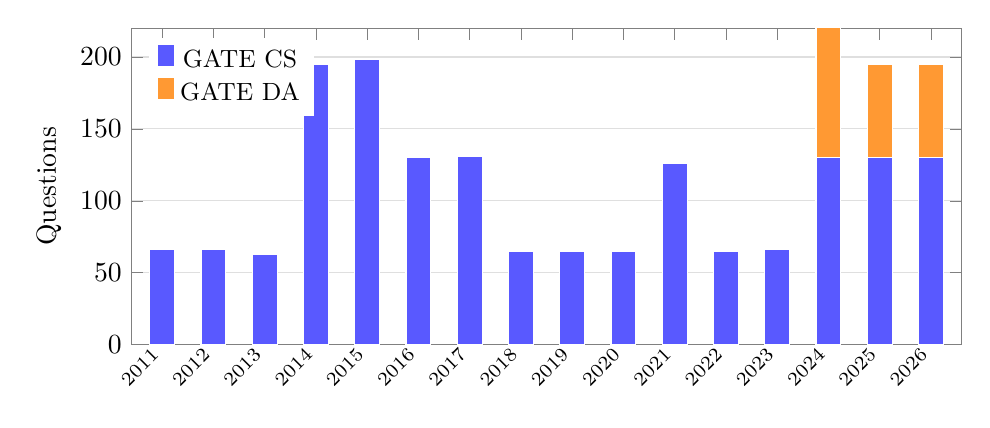
\begin{tikzpicture}
\begin{axis}[ybar stacked, width=\textwidth, height=5.6cm, bar width=9pt, ymin=0, ymax=220,
  symbolic x coords={2011,2012,2013,2014,2015,2016,2017,2018,2019,2020,2021,2022,2023,2024,2025,2026},
  xtick=data, x tick label style={rotate=45, anchor=east, font=\scriptsize}, ylabel={Questions},
  ymajorgrids, grid style={gray!25}, axis line style={gray}, legend style={at={(0.02,0.97)}, anchor=north west, font=\small, draw=none},
  enlarge x limits=0.04]
\addplot[fill=blue!65, draw=white] coordinates {(2011,66)(2012,66)(2013,63)(2014,195)(2015,198)(2016,130)(2017,131)(2018,65)(2019,65)(2020,65)(2021,126)(2022,65)(2023,66)(2024,130)(2025,130)(2026,130)};
\addplot[fill=orange!80, draw=white] coordinates {(2011,0)(2012,0)(2013,0)(2014,0)(2015,0)(2016,0)(2017,0)(2018,0)(2019,0)(2020,0)(2021,0)(2022,0)(2023,0)(2024,120)(2025,65)(2026,65)};
\legend{GATE CS, GATE DA}
\end{axis}
\end{tikzpicture}
\caption{Questions in the corpus per year (multi-session years contain two or three papers)}
\label{fig:peryear}
\end{figure}

\section{Historical Analysis}
\subsection{Subject weightage}
Figure~\ref{fig:cs-weight} shows the average marks per paper of each GATE CS subject over sixteen years. General
Aptitude contributes a fixed 15 marks; among technical subjects Algorithms (10.3) and Programming and Data Structures
(9.8) lead, followed by Discrete Mathematics (8.3) and Operating Systems (7.7), while Calculus (2.4) and Linear Algebra
(3.0) carry the least. All CS subjects are classified as stable---GATE CS has not shifted its subject balance in a
measurable way since 2011. GATE DA (Figure~\ref{fig:da-weight}) is dominated by Probability and Statistics (18.5 marks,
19.2\%), which is also rising, followed by Programming/Data Structures/Algorithms and Machine Learning; with only three
years of data the DA trends should be read as indicative.

\begin{figure}[h]
\centering
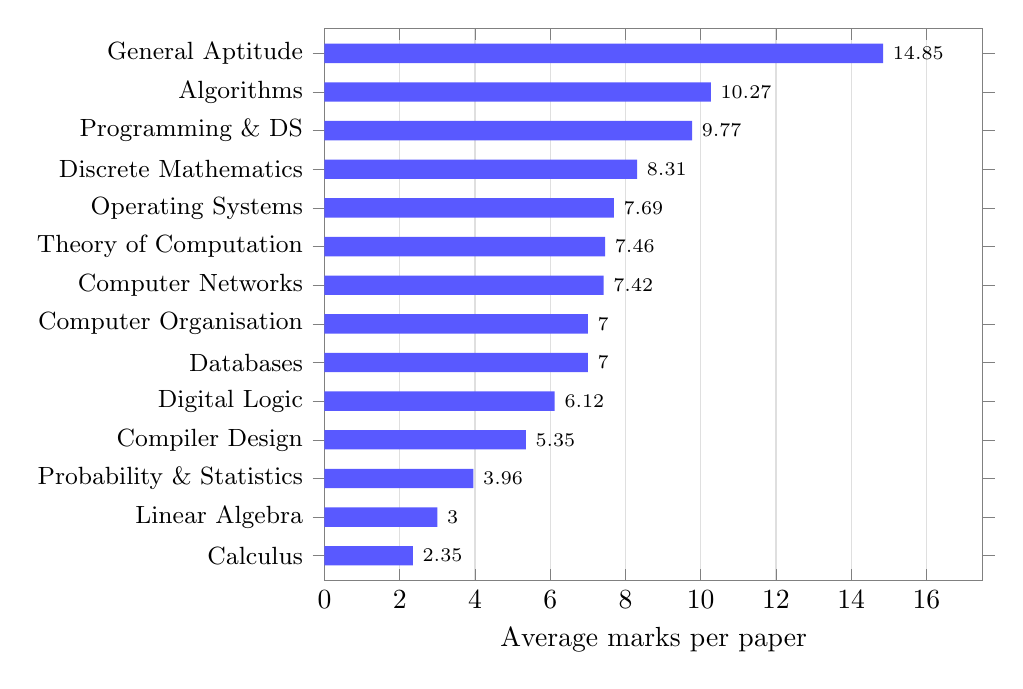
\begin{tikzpicture}
\begin{axis}[xbar, width=0.82\textwidth, height=8.6cm, bar width=7pt, xmin=0, xmax=17.5,
  symbolic y coords={Calculus,Linear Algebra,Probability \& Statistics,Compiler Design,Digital Logic,Databases,
    Computer Organisation,Computer Networks,Theory of Computation,Operating Systems,Discrete Mathematics,
    Programming \& DS,Algorithms,General Aptitude},
  ytick=data, y tick label style={font=\small}, xlabel={Average marks per paper}, nodes near coords,
  nodes near coords style={font=\scriptsize}, xmajorgrids, grid style={gray!25}, axis line style={gray}, enlarge y limits=0.05]
\addplot[fill=blue!65, draw=none] coordinates {(2.35,Calculus)(3.0,Linear Algebra)(3.96,Probability \& Statistics)(5.35,Compiler Design)
  (6.12,Digital Logic)(7.0,Databases)(7.0,Computer Organisation)(7.42,Computer Networks)(7.46,Theory of Computation)
  (7.69,Operating Systems)(8.31,Discrete Mathematics)(9.77,Programming \& DS)(10.27,Algorithms)(14.85,General Aptitude)};
\end{axis}
\end{tikzpicture}
\caption{GATE CS subject weightage, 2011--2026 (26 papers)}
\label{fig:cs-weight}
\end{figure}

\begin{figure}[h]
\centering
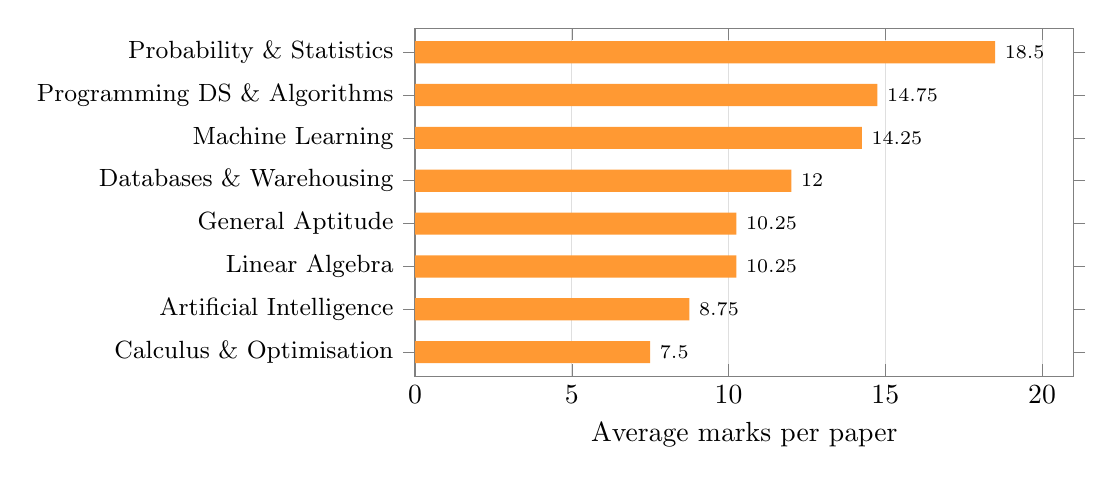
\begin{tikzpicture}
\begin{axis}[xbar, width=0.82\textwidth, height=6cm, bar width=8pt, xmin=0, xmax=21,
  symbolic y coords={Calculus \& Optimisation,Artificial Intelligence,Linear Algebra,General Aptitude,Databases \& Warehousing,
    Machine Learning,Programming DS \& Algorithms,Probability \& Statistics},
  ytick=data, y tick label style={font=\small}, xlabel={Average marks per paper}, nodes near coords,
  nodes near coords style={font=\scriptsize}, xmajorgrids, grid style={gray!25}, axis line style={gray}, enlarge y limits=0.08]
\addplot[fill=orange!80, draw=none] coordinates {(7.5,Calculus \& Optimisation)(8.75,Artificial Intelligence)(10.25,Linear Algebra)
  (10.25,General Aptitude)(12.0,Databases \& Warehousing)(14.25,Machine Learning)(14.75,Programming DS \& Algorithms)(18.5,Probability \& Statistics)};
\end{axis}
\end{tikzpicture}
\caption{GATE DA subject weightage, 2024--2026 (including the official sample)}
\label{fig:da-weight}
\end{figure}

\subsection{Hot topics}
Table~\ref{tab:hot-cs} lists the ten hottest GATE CS topics by Eq.~\ref{eq:hot}. Apart from the aptitude topics,
programming in C and recursion, the memory hierarchy, graph algorithms, virtual memory, trees and heaps, finite automata
and relational algebra/SQL each appeared in all or all but one of the sixteen years. For DA
(Table~\ref{tab:hot-da}) file organisation and indexing, random variables and their distributions, and classification
methods lead.

\begin{table}[h]
\centering
\caption{Ten hottest GATE CS topics}
\label{tab:hot-cs}
\small
\begin{tabularx}{\textwidth}{@{}Xlccc@{}}
\toprule
\textbf{Topic} & \textbf{Subject} & \textbf{Hot} & \textbf{Marks/paper} & \textbf{Years}\\
\midrule
Verbal aptitude & General Aptitude & 100.0 & 7.42 & 16/16\\
Programming in C and recursion & Prog.\ \& DS & 81.1 & 4.69 & 16/16\\
Quantitative aptitude & General Aptitude & 67.9 & 4.35 & 15/16\\
Memory hierarchy: cache, main and secondary memory & COA & 62.1 & 3.00 & 15/16\\
Graph traversals, MST and shortest paths & Algorithms & 60.7 & 2.77 & 16/16\\
Memory management and virtual memory & Operating Systems & 57.2 & 2.46 & 16/16\\
Trees, BSTs and binary heaps & Prog.\ \& DS & 56.9 & 2.73 & 16/16\\
Spatial aptitude & General Aptitude & 53.5 & 1.88 & 11/16\\
Regular expressions and finite automata & TOC & 49.2 & 2.58 & 16/16\\
Relational algebra, tuple calculus, SQL & Databases & 47.9 & 2.92 & 16/16\\
\bottomrule
\end{tabularx}
\end{table}

\begin{table}[h]
\centering
\caption{Six hottest GATE DA topics}
\label{tab:hot-da}
\small
\begin{tabularx}{\textwidth}{@{}Xlcc@{}}
\toprule
\textbf{Topic} & \textbf{Subject} & \textbf{Hot} & \textbf{Marks/paper}\\
\midrule
File organisation and indexing & Databases \& Warehousing & 100.0 & 5.50\\
Discrete and continuous random variables & Probability \& Statistics & 94.1 & 6.50\\
Verbal aptitude & General Aptitude & 86.5 & 4.50\\
Mean, variance, covariance, correlation & Probability \& Statistics & 79.8 & 4.75\\
Classification (LR, k-NN, naive Bayes, LDA, SVM, trees) & Machine Learning & 72.9 & 5.75\\
Programming in Python & Prog., DS \& Algorithms & 70.5 & 4.75\\
\bottomrule
\end{tabularx}
\end{table}

\subsection{Question types, cognitive levels and recurrence}
Averaged over all years, a GATE CS paper contains 36.5 MCQ, 23.4 NAT and 5.2 MSQ questions (MSQ was introduced only
in 2021), with 29.5 one-mark and 35.5 two-mark questions; DA papers have markedly more MSQ (11.0 per paper).
Figure~\ref{fig:bloom} compares the Bloom distribution: CS questions are dominated by \emph{Understand} and \emph{Apply},
whereas DA places more weight on \emph{Apply} and \emph{Analyze}. About 10\% of questions in both papers depend on a
figure, which text-based generation cannot reproduce.

\begin{figure}[h]
\centering
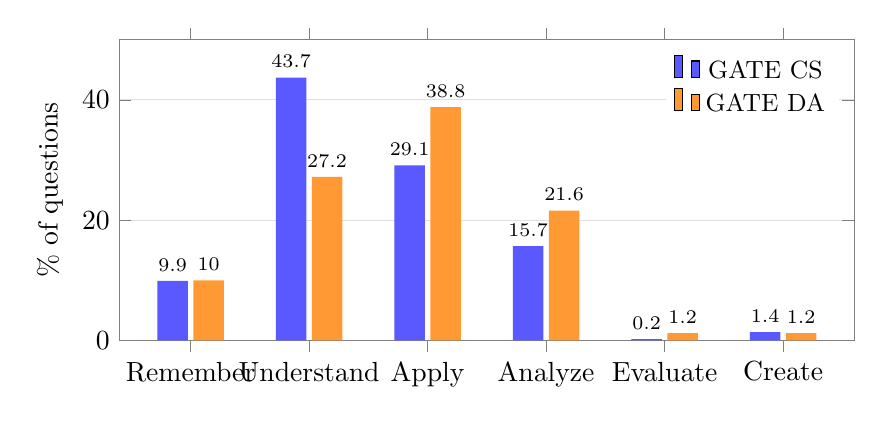
\begin{tikzpicture}
\begin{axis}[ybar, width=0.9\textwidth, height=5.4cm, bar width=11pt, ymin=0, ymax=50,
  symbolic x coords={Remember,Understand,Apply,Analyze,Evaluate,Create}, xtick=data, ylabel={\% of questions},
  nodes near coords, nodes near coords style={font=\scriptsize}, ymajorgrids, grid style={gray!25}, axis line style={gray},
  legend style={at={(0.98,0.97)}, anchor=north east, font=\small, draw=none}, enlarge x limits=0.12]
\addplot[fill=blue!65, draw=none] coordinates {(Remember,9.9)(Understand,43.7)(Apply,29.1)(Analyze,15.7)(Evaluate,0.2)(Create,1.4)};
\addplot[fill=orange!80, draw=none] coordinates {(Remember,10.0)(Understand,27.2)(Apply,38.8)(Analyze,21.6)(Evaluate,1.2)(Create,1.2)};
\legend{GATE CS, GATE DA}
\end{axis}
\end{tikzpicture}
\caption{Bloom's taxonomy distribution of past questions}
\label{fig:bloom}
\end{figure}

Recurrence analysis found concept-level repetition rather than verbatim copying (Table~\ref{tab:recur}): shortest
remaining time first (SRTF) scheduling with arrival times was set in 2014, 2016, 2017 and 2019 with only the numbers
changed, and a multi-layer perceptron parameter-count question in the official DA sample re-appeared in the 2026 paper.
An early version of the analysis compared stems only and reported spurious ``repeats'' between generic stems such as
``Which of the following statements is FALSE?''; including the options removed these false positives.

\begin{table}[h]
\centering
\caption{Most similar question pairs across years}
\label{tab:recur}
\small
\begin{tabularx}{\textwidth}{@{}clX@{}}
\toprule
\textbf{Sim.} & \textbf{Papers} & \textbf{Concept}\\
\midrule
0.86 & 2014 CS3 Q43 -- 2017 CS1 Q24 & SRTF scheduling: average waiting time with arrival times\\
0.81 & 2014 CS3 Q43 -- 2019 CS Q51 & SRTF scheduling\\
0.81 & 2017 CS1 Q24 -- 2019 CS Q51 & SRTF scheduling\\
0.73 & 2016 CS2 Q57 -- 2017 CS1 Q24 & Pre-emptive scheduling with arrival and burst times\\
0.66 & 2024 DA (sample) Q53 -- 2026 DA Q56 & MLP with one hidden layer: number of parameters\\
\bottomrule
\end{tabularx}
\end{table}

\section{Topic Classifier Evaluation}
The classifiers were evaluated against the teacher's labels on the 2026 papers, which were excluded from training
(Table~\ref{tab:clf}, Figure~\ref{fig:clf}). For GATE CS (130 test questions, 58 topics present, 1,545 training
questions) the distilled TF-IDF + LR student reaches 77.7\% topic accuracy (macro-F1 0.731) and 88.5\% subject
accuracy, about five points above the zero-shot sentence-embedding matcher and far above the majority-class baseline.
The value of data is visible in the earliest configuration: trained on a single year of zero-shot labels the same model
reached only 43.8\%. For GATE DA, with only 185 training questions, the student merely ties zero-shot on topics and is
worse on subjects; DA will benefit as more papers are released. The practical advantage of the student is its footprint:
it needs no neural network at run time and labels a paper in milliseconds on the 512\,MB server.

\begin{table}[h]
\centering
\caption{Topic classification on held-out 2026 papers (accuracy, \%)}
\label{tab:clf}
\small
\begin{tabular}{@{}lcccc@{}}
\toprule
& \multicolumn{2}{c}{\textbf{GATE CS} (n = 130)} & \multicolumn{2}{c}{\textbf{GATE DA} (n = 65)}\\
\cmidrule(lr){2-3}\cmidrule(l){4-5}
\textbf{Method} & Topic & Subject & Topic & Subject\\
\midrule
Majority class & 3.8 & 11.5 & 3.1 & 21.5\\
Zero-shot (MiniLM embeddings) & 73.1 & 83.1 & 44.6 & \textbf{81.5}\\
Student, 1 year of zero-shot labels & 43.8 & 56.2 & 38.5 & 58.5\\
\textbf{Student, all years of LLM labels} & \textbf{77.7} & \textbf{88.5} & \textbf{44.6} & 75.4\\
\bottomrule
\end{tabular}
\end{table}

\begin{figure}[h]
\centering
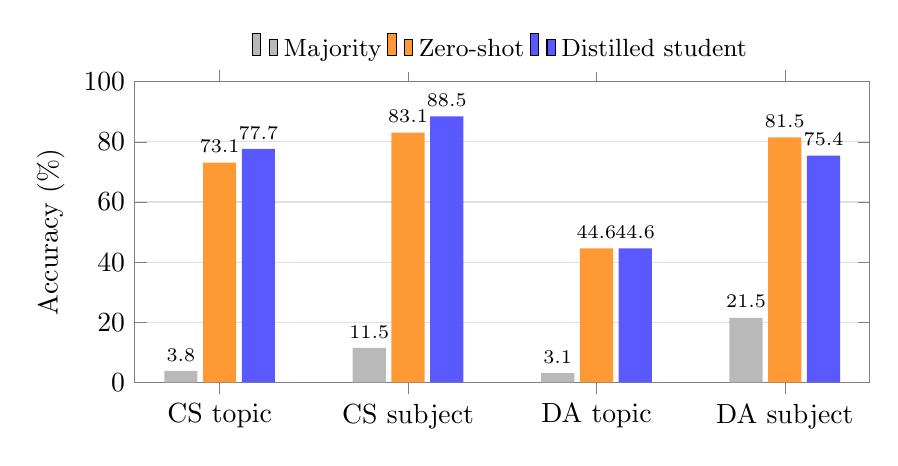
\begin{tikzpicture}
\begin{axis}[ybar, width=0.9\textwidth, height=5.4cm, bar width=12pt, ymin=0, ymax=100,
  symbolic x coords={CS topic,CS subject,DA topic,DA subject}, xtick=data, ylabel={Accuracy (\%)},
  nodes near coords, nodes near coords style={font=\scriptsize}, ymajorgrids, grid style={gray!25}, axis line style={gray},
  legend style={at={(0.5,1.03)}, anchor=south, legend columns=3, font=\small, draw=none}, enlarge x limits=0.15]
\addplot[fill=gray!55, draw=none] coordinates {(CS topic,3.8)(CS subject,11.5)(DA topic,3.1)(DA subject,21.5)};
\addplot[fill=orange!80, draw=none] coordinates {(CS topic,73.1)(CS subject,83.1)(DA topic,44.6)(DA subject,81.5)};
\addplot[fill=blue!65, draw=none] coordinates {(CS topic,77.7)(CS subject,88.5)(DA topic,44.6)(DA subject,75.4)};
\legend{Majority, Zero-shot, Distilled student}
\end{axis}
\end{tikzpicture}
\caption{Classifier comparison on held-out 2026 papers}
\label{fig:clf}
\end{figure}

\section{Paper Generation}
\subsection{Validation results}
Table~\ref{tab:gen} summarises representative generation runs. All papers met their question count and marks total.
Generated questions were novel: the maximum similarity of any generated question to any of the 1,971 past questions
was between 0.43 and 0.69, below the threshold $\theta=0.8$, and the mean for the full mock was 0.33. The blind
re-solving stage rejected one key in each of the two runs where it was active; in one case the regenerated question
passed, in the other the slot fell back to a real past question.

\begin{table}[h]
\centering
\caption{Generation runs and their validation reports}
\label{tab:gen}
\small
\begin{tabularx}{\textwidth}{@{}Xccccc@{}}
\toprule
\textbf{Request} & \textbf{Qs} & \textbf{Marks} & \textbf{Max sim.} & \textbf{Keys fixed} & \textbf{Time}\\
\midrule
GATE CS full mock test$^{\dagger}$ & 65/65 & 100 \checkmark & 0.61 & -- & 3 min 7 s\\
Mid-sem paper for DBMS & 10/10 & 30 \checkmark & 0.43 & -- (descriptive) & --\\
6 questions on operating systems$^{\dagger}$ & 6/6 & 9 \checkmark & 0.48 & -- & --\\
4 questions on deadlock for GATE CS & 4/4 & 6 \checkmark & 0.69 & 1 regenerated & --\\
2 questions on cache memory (deployed server) & 2/2 & 3 \checkmark & 0.63 & 1 $\rightarrow$ PYQ & 46 s\\
\bottomrule
\multicolumn{6}{@{}l}{\footnotesize $^{\dagger}$Run before the verification stage was added.}
\end{tabularx}
\end{table}

\subsection{Faithfulness to the examination pattern}
Figure~\ref{fig:faith} compares the marks per subject in the generated GATE CS mock with the sixteen-year averages. The
Pearson correlation is 0.81 and the mean absolute difference is 2.0 marks per subject; deviations come from sampling a
single paper (for instance no Probability and Statistics question was drawn), as happens between real papers too. The
mock contains 38 MCQ, 22 NAT and 5 MSQ questions, close to the recent pattern in the keys.

\begin{figure}[h]
\centering
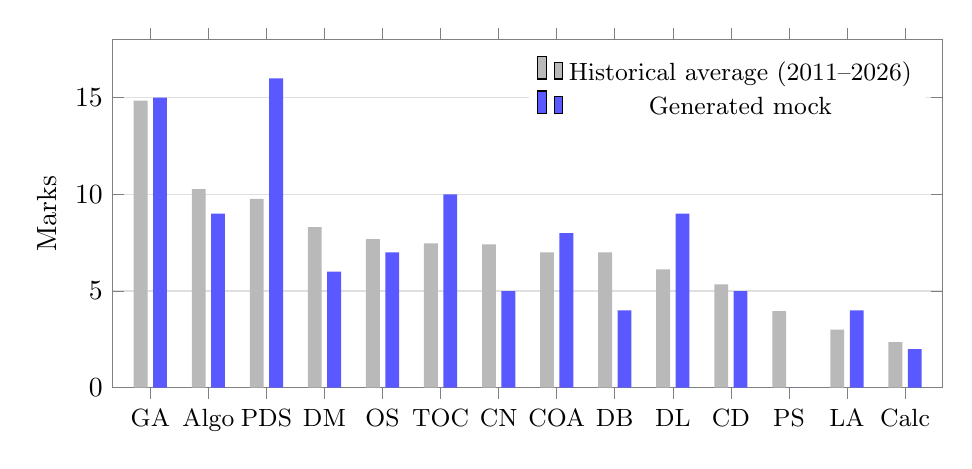
\begin{tikzpicture}
\begin{axis}[ybar, width=\textwidth, height=6cm, bar width=5pt, ymin=0, ymax=18,
  symbolic x coords={GA,Algo,PDS,DM,OS,TOC,CN,COA,DB,DL,CD,PS,LA,Calc}, xtick=data, ylabel={Marks},
  ymajorgrids, grid style={gray!25}, axis line style={gray}, x tick label style={font=\small},
  legend style={at={(0.98,0.97)}, anchor=north east, font=\small, draw=none}, enlarge x limits=0.05]
\addplot[fill=gray!55, draw=none] coordinates {(GA,14.85)(Algo,10.27)(PDS,9.77)(DM,8.31)(OS,7.69)(TOC,7.46)(CN,7.42)(COA,7.0)(DB,7.0)(DL,6.12)(CD,5.35)(PS,3.96)(LA,3.0)(Calc,2.35)};
\addplot[fill=blue!65, draw=none] coordinates {(GA,15)(Algo,9)(PDS,16)(DM,6)(OS,7)(TOC,10)(CN,5)(COA,8)(DB,4)(DL,9)(CD,5)(PS,0)(LA,4)(Calc,2)};
\legend{Historical average (2011--2026), Generated mock}
\end{axis}
\end{tikzpicture}
\caption{Subject marks of a generated GATE CS mock against the historical average ($r=0.81$)}
\label{fig:faith}
\end{figure}

\subsection{Quality of generated questions}
Generated questions are GATE-like in style and depth: multi-step numerical problems (paging, semaphores, inode block
counts), statement-evaluation MSQs, and LaTeX-formatted mathematics. Two questions from an early run were checked by
hand and both keys were correct (a counting semaphore with 18 \texttt{wait} operations and five blocked processes giving
$m=9$ \texttt{signal} operations, and an 18\,MB file needing 4,614 blocks with one single- and one double-indirect
pointer). The same testing also surfaced a Banker's-algorithm question with \emph{no} correct option, whose key the
tutor's own explanation contradicted---the incident that led to the blind verification stage. Sample papers are
reproduced in Appendix~\ref{app:outputs}.

\section{Study Assistant}
In a scripted session (Appendix~\ref{app:outputs}) the assistant answered ``Which subjects should I prioritise for GATE
DA?'' with the exact weightage table from the corpus (2024--2026) rather than generic advice, created a deadlock practice
set and asked its questions one at a time, fetched the official key only after the student's answer, explained the
Banker's-algorithm solution step by step and recorded the attempt, after which \texttt{my\_progress} reported the topic
with priority 19.7. Two failure modes were found and fixed: requests named a topic (``deadlock'') but were resolved only
to its subject, producing off-topic questions---topic-level focus was added to the request schema; and a temporary
``model overloaded'' error aborted the conversation---such errors now fall through to the next model.

\section{Deployed Application}
The application is deployed at \url{https://papermind-pmbz.onrender.com} and redeploys on every push to the GitHub
repository. On the free tier the first request after 15 idle minutes takes 30--60 seconds while the service wakes; the
first analysis of an area takes about 15 seconds and is cached afterwards; generation time is dominated by the LLM and
matches local runs. Table~\ref{tab:api} lists the REST endpoints and Figures~\ref{fig:ui-gen}--\ref{fig:ui-chat} show the
interface.

\begin{table}[h]
\centering
\caption{REST API}
\label{tab:api}
\small
\begin{tabularx}{\textwidth}{@{}llX@{}}
\toprule
\textbf{Method} & \textbf{Endpoint} & \textbf{Purpose}\\
\midrule
GET & \texttt{/api/health} & Status, LLM availability, syllabus areas\\
GET, POST & \texttt{/api/papers} & List corpus / upload a PDF or page photos\\
DELETE & \texttt{/api/papers/\{id\}} & Remove a paper\\
GET & \texttt{/api/questions} & Past questions by area, unit, topic\\
GET & \texttt{/api/analysis/\{area\}} & Historical analysis report\\
POST & \texttt{/api/generate} & Generate a paper from a free-text request\\
GET & \texttt{/api/generated[/\{id\}]} & Previously generated papers\\
GET, POST, DELETE & \texttt{/api/chat} & Assistant history / message / reset\\
GET & \texttt{/api/progress} & A student's accuracy and study priorities\\
\bottomrule
\end{tabularx}
\end{table}

\newcommand{\shot}[3]{%
  \begin{figure}[p]\centering
  \IfFileExists{figures/#1.png}{\includegraphics[width=\textwidth,height=0.78\textheight,keepaspectratio]{figures/#1.png}}%
    {\fbox{\parbox{0.9\textwidth}{\centering\vspace{2cm}Screenshot \texttt{figures/#1.png}\vspace{2cm}}}}
  \caption{#2}\label{#3}\end{figure}}
\shot{ui_paper}{Generate tab: a generated GATE CS mock test rendered with KaTeX}{fig:ui-gen}
\shot{ui_paper_answers}{Generated mid-semester paper with answers and marking schemes shown}{fig:ui-ans}
\shot{ui_insights}{Insights tab: subject weightage, hot topics and recurring concepts for GATE CS}{fig:ui-ins}
\shot{ui_assistant}{Assistant tab: grounded advice, quiz and progress panel}{fig:ui-chat}

\section{Discussion and Limitations}
\begin{itemize}
  \item \textbf{Verification is not proof.} Blind re-solving catches keys on which two independent solutions disagree,
        but a question on which both are wrong in the same way can pass.
  \item \textbf{Figures.} About 10\% of past questions depend on diagrams, which are neither reproduced in the corpus
        text nor generated.
  \item \textbf{Label quality.} The classifier is evaluated against LLM labels, not human annotation; reported accuracy
        measures agreement with the teacher.
  \item \textbf{OCR noise.} Scanned years contain a few missed or merged questions (for example 60 instead of 65 in one
        2021 session).
  \item \textbf{Free-tier limits.} About 20 Gemini requests per model per day and a sleeping, ephemeral free server
        constrain heavy use; uploaded papers and progress reset when the server restarts.
\end{itemize}

\section{Chapter Summary}
A 31-paper, 1,971-question corpus was built and analysed, yielding interpretable subject weightage, hot topics,
question-type and cognitive-level distributions, and concept recurrence. The distilled topic classifier reached 77.7\%
topic and 88.5\% subject accuracy on unseen GATE CS papers. Generated papers met every structural constraint, were novel
with respect to past papers, tracked the historical subject distribution ($r=0.81$), and had their answer keys
independently verified. The assistant and web application make these capabilities available to students at no cost.
